\documentclass{article}
\usepackage{graphicx}
\usepackage[margin=1in]{geometry} % For reasonable margins
\usepackage{caption} % For better caption control

\title{Analysis Figures Report}
\author{Generated by AI}
\date{\today}

\begin{document}

\maketitle
\newpage

\section{Doctor Questions Count}
\begin{figure}[h!]
    \centering
    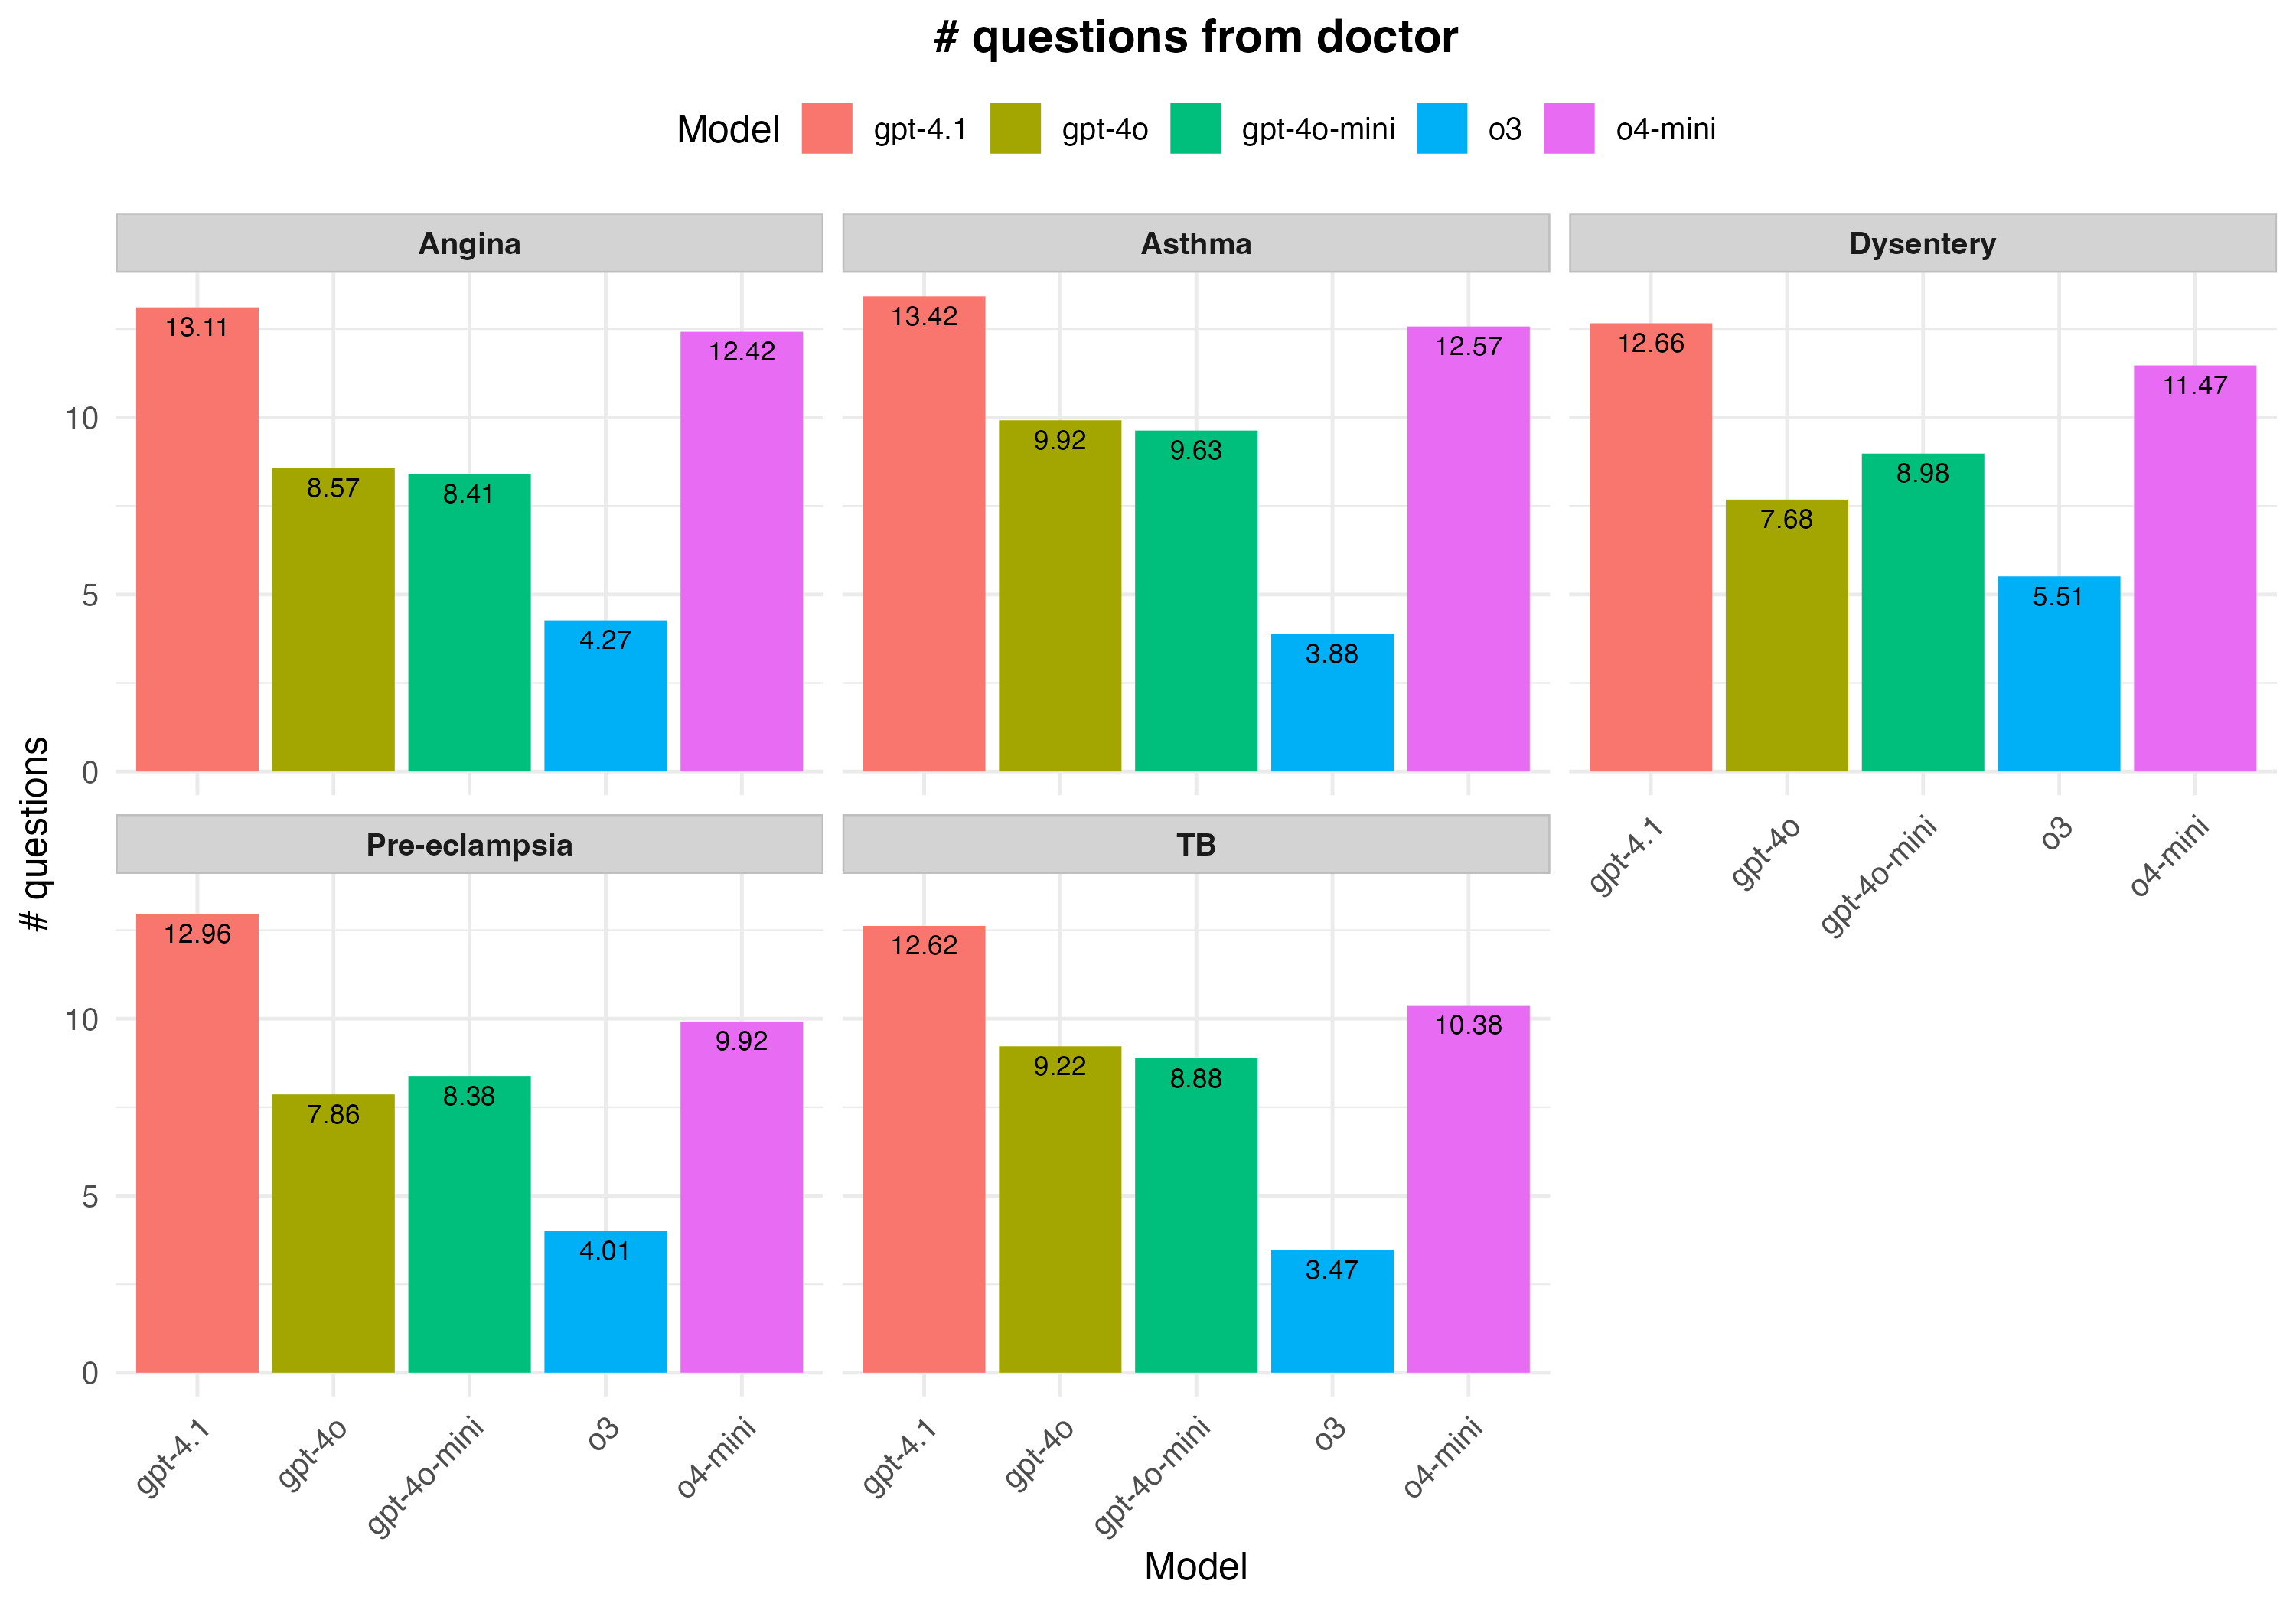
\includegraphics[width=0.9\textwidth]{figs/doctor_questions_count_plot.png}
    \caption{Bar plot of the number of questions from the doctor, faceted by case.}
    \label{fig:doc_questions}
\end{figure}
\newpage

\section{Checklist Completion Rate}
\begin{figure}[h!]
    \centering
    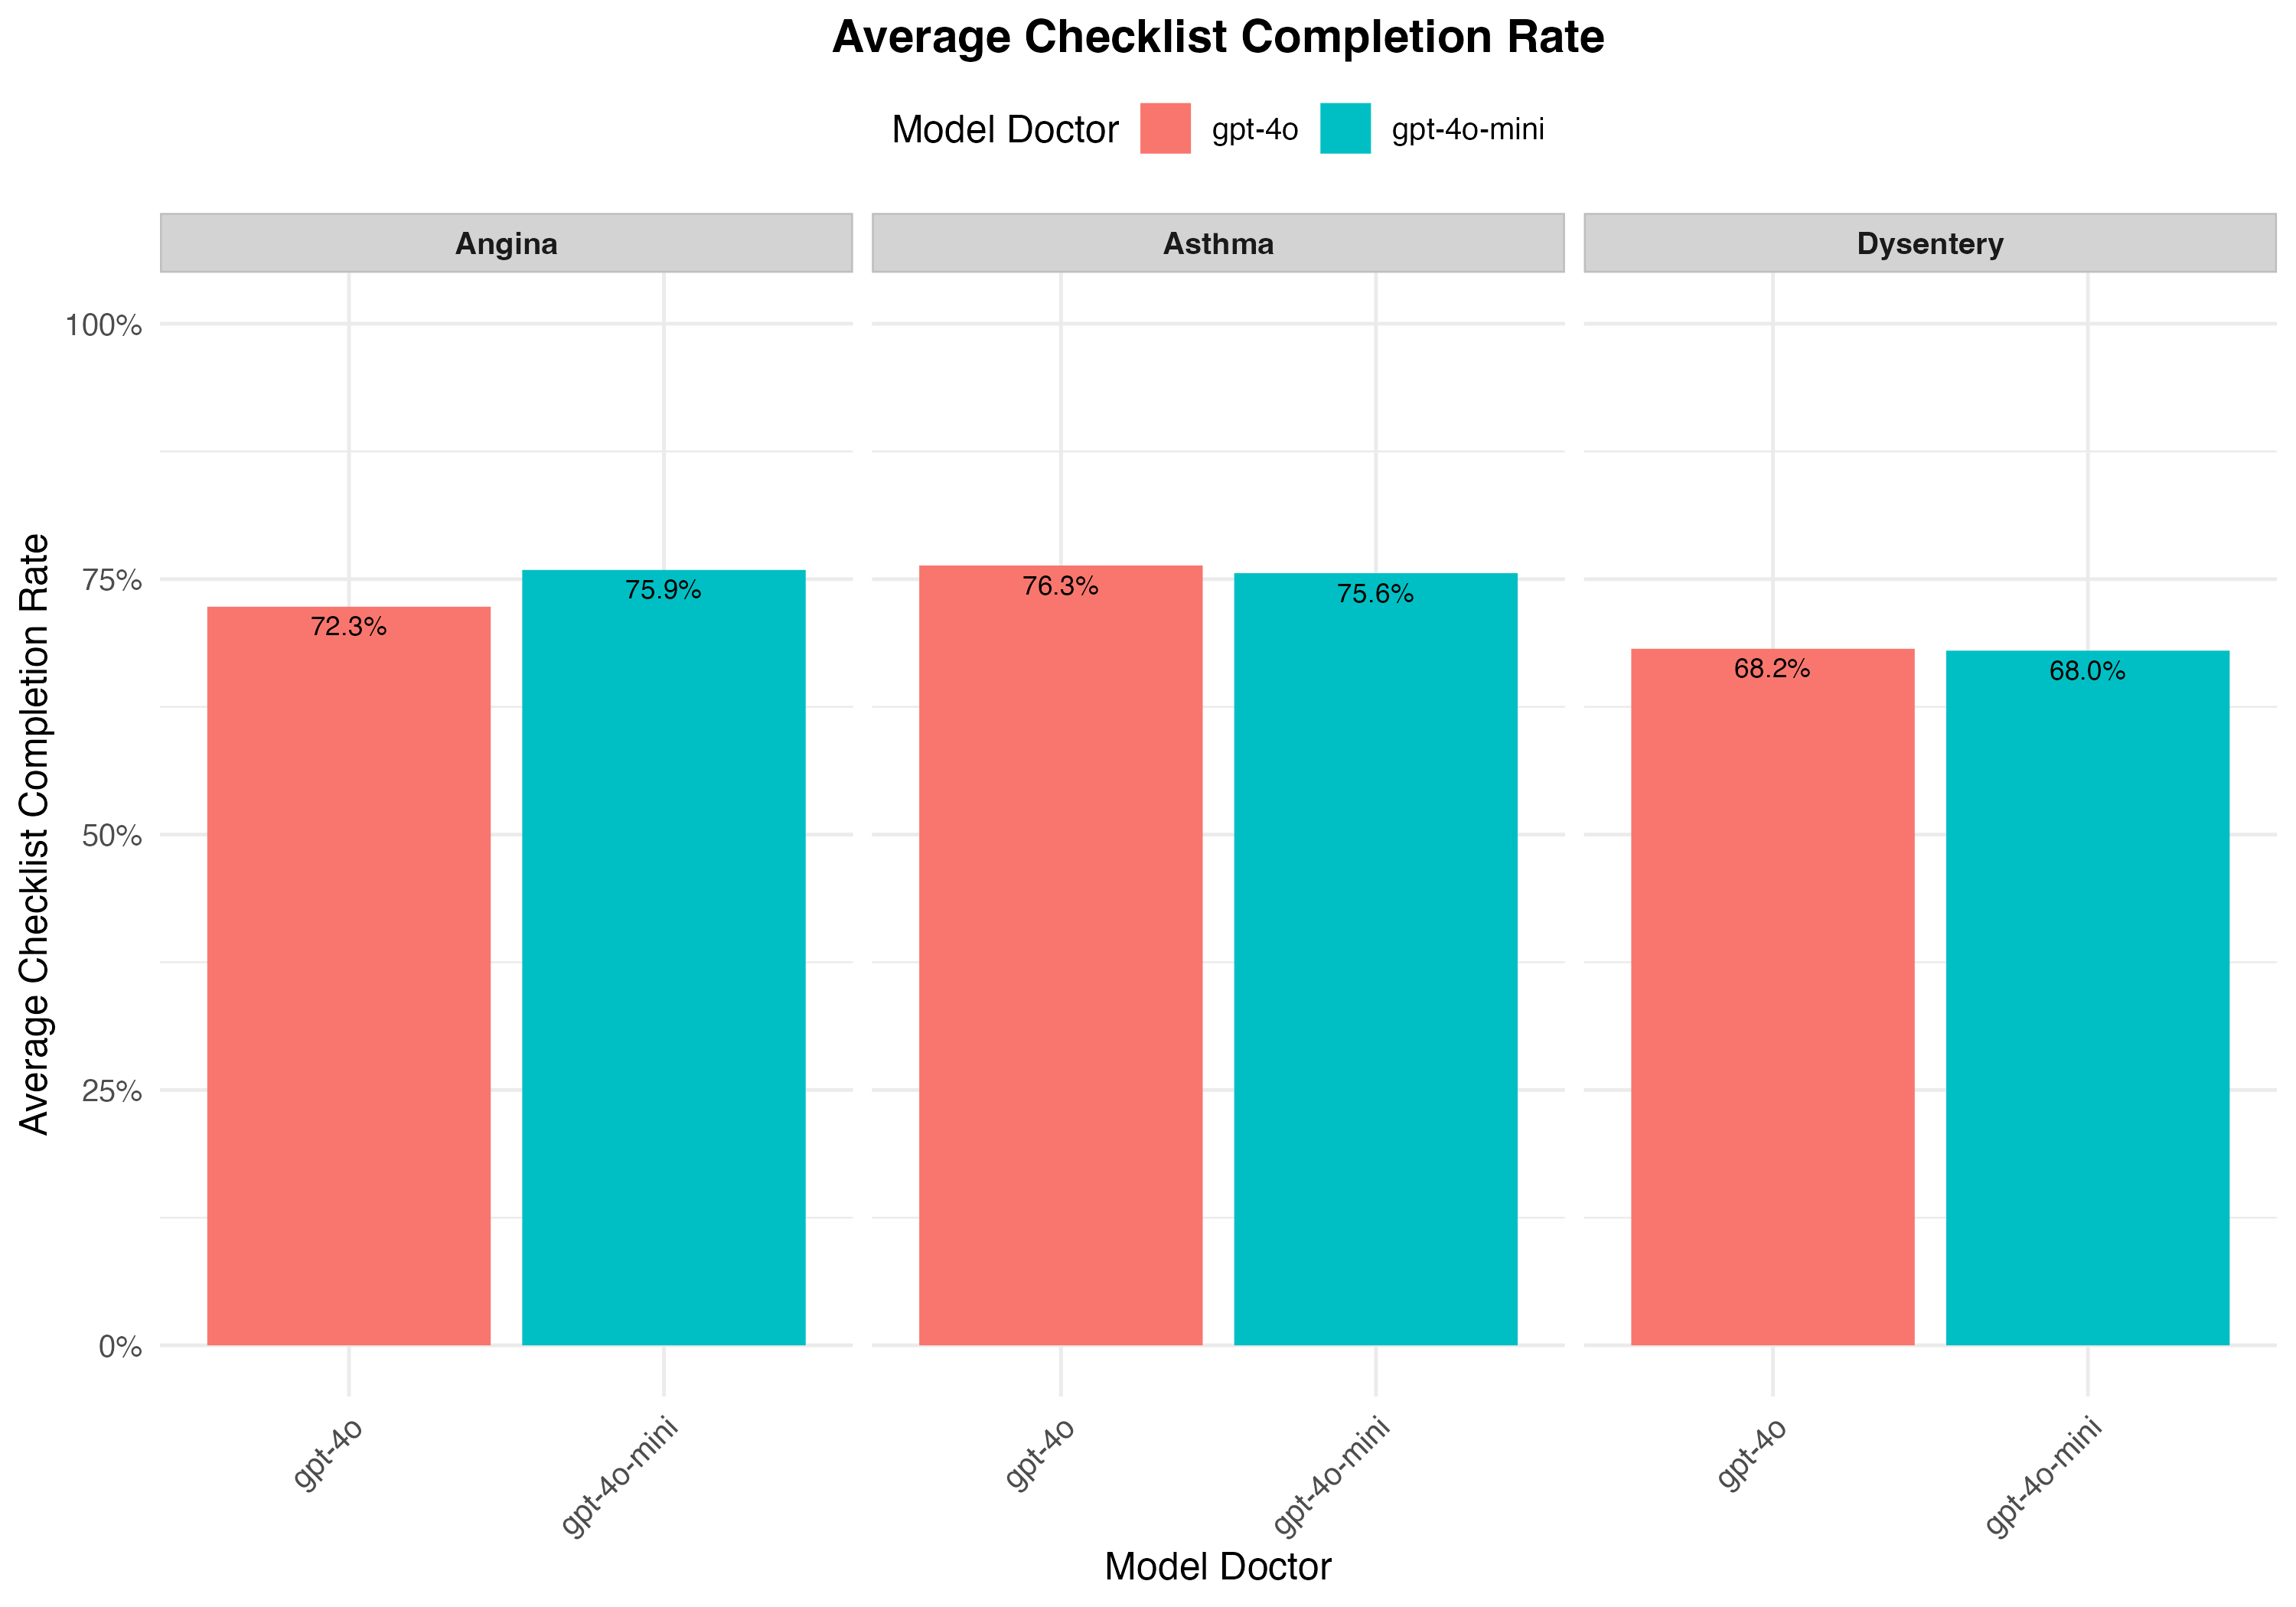
\includegraphics[width=0.9\textwidth]{figs/checklist_completion_rate_plot.png}
    \caption{Bar plot of the average checklist completion rate, faceted by case. Note: Pre-eclampsia and TB cases are filtered out.}
    \label{fig:checklist_completion}
\end{figure}
\newpage

\section{Doctor Questions Without IDs (Off-Script)}
\begin{figure}[h!]
    \centering
    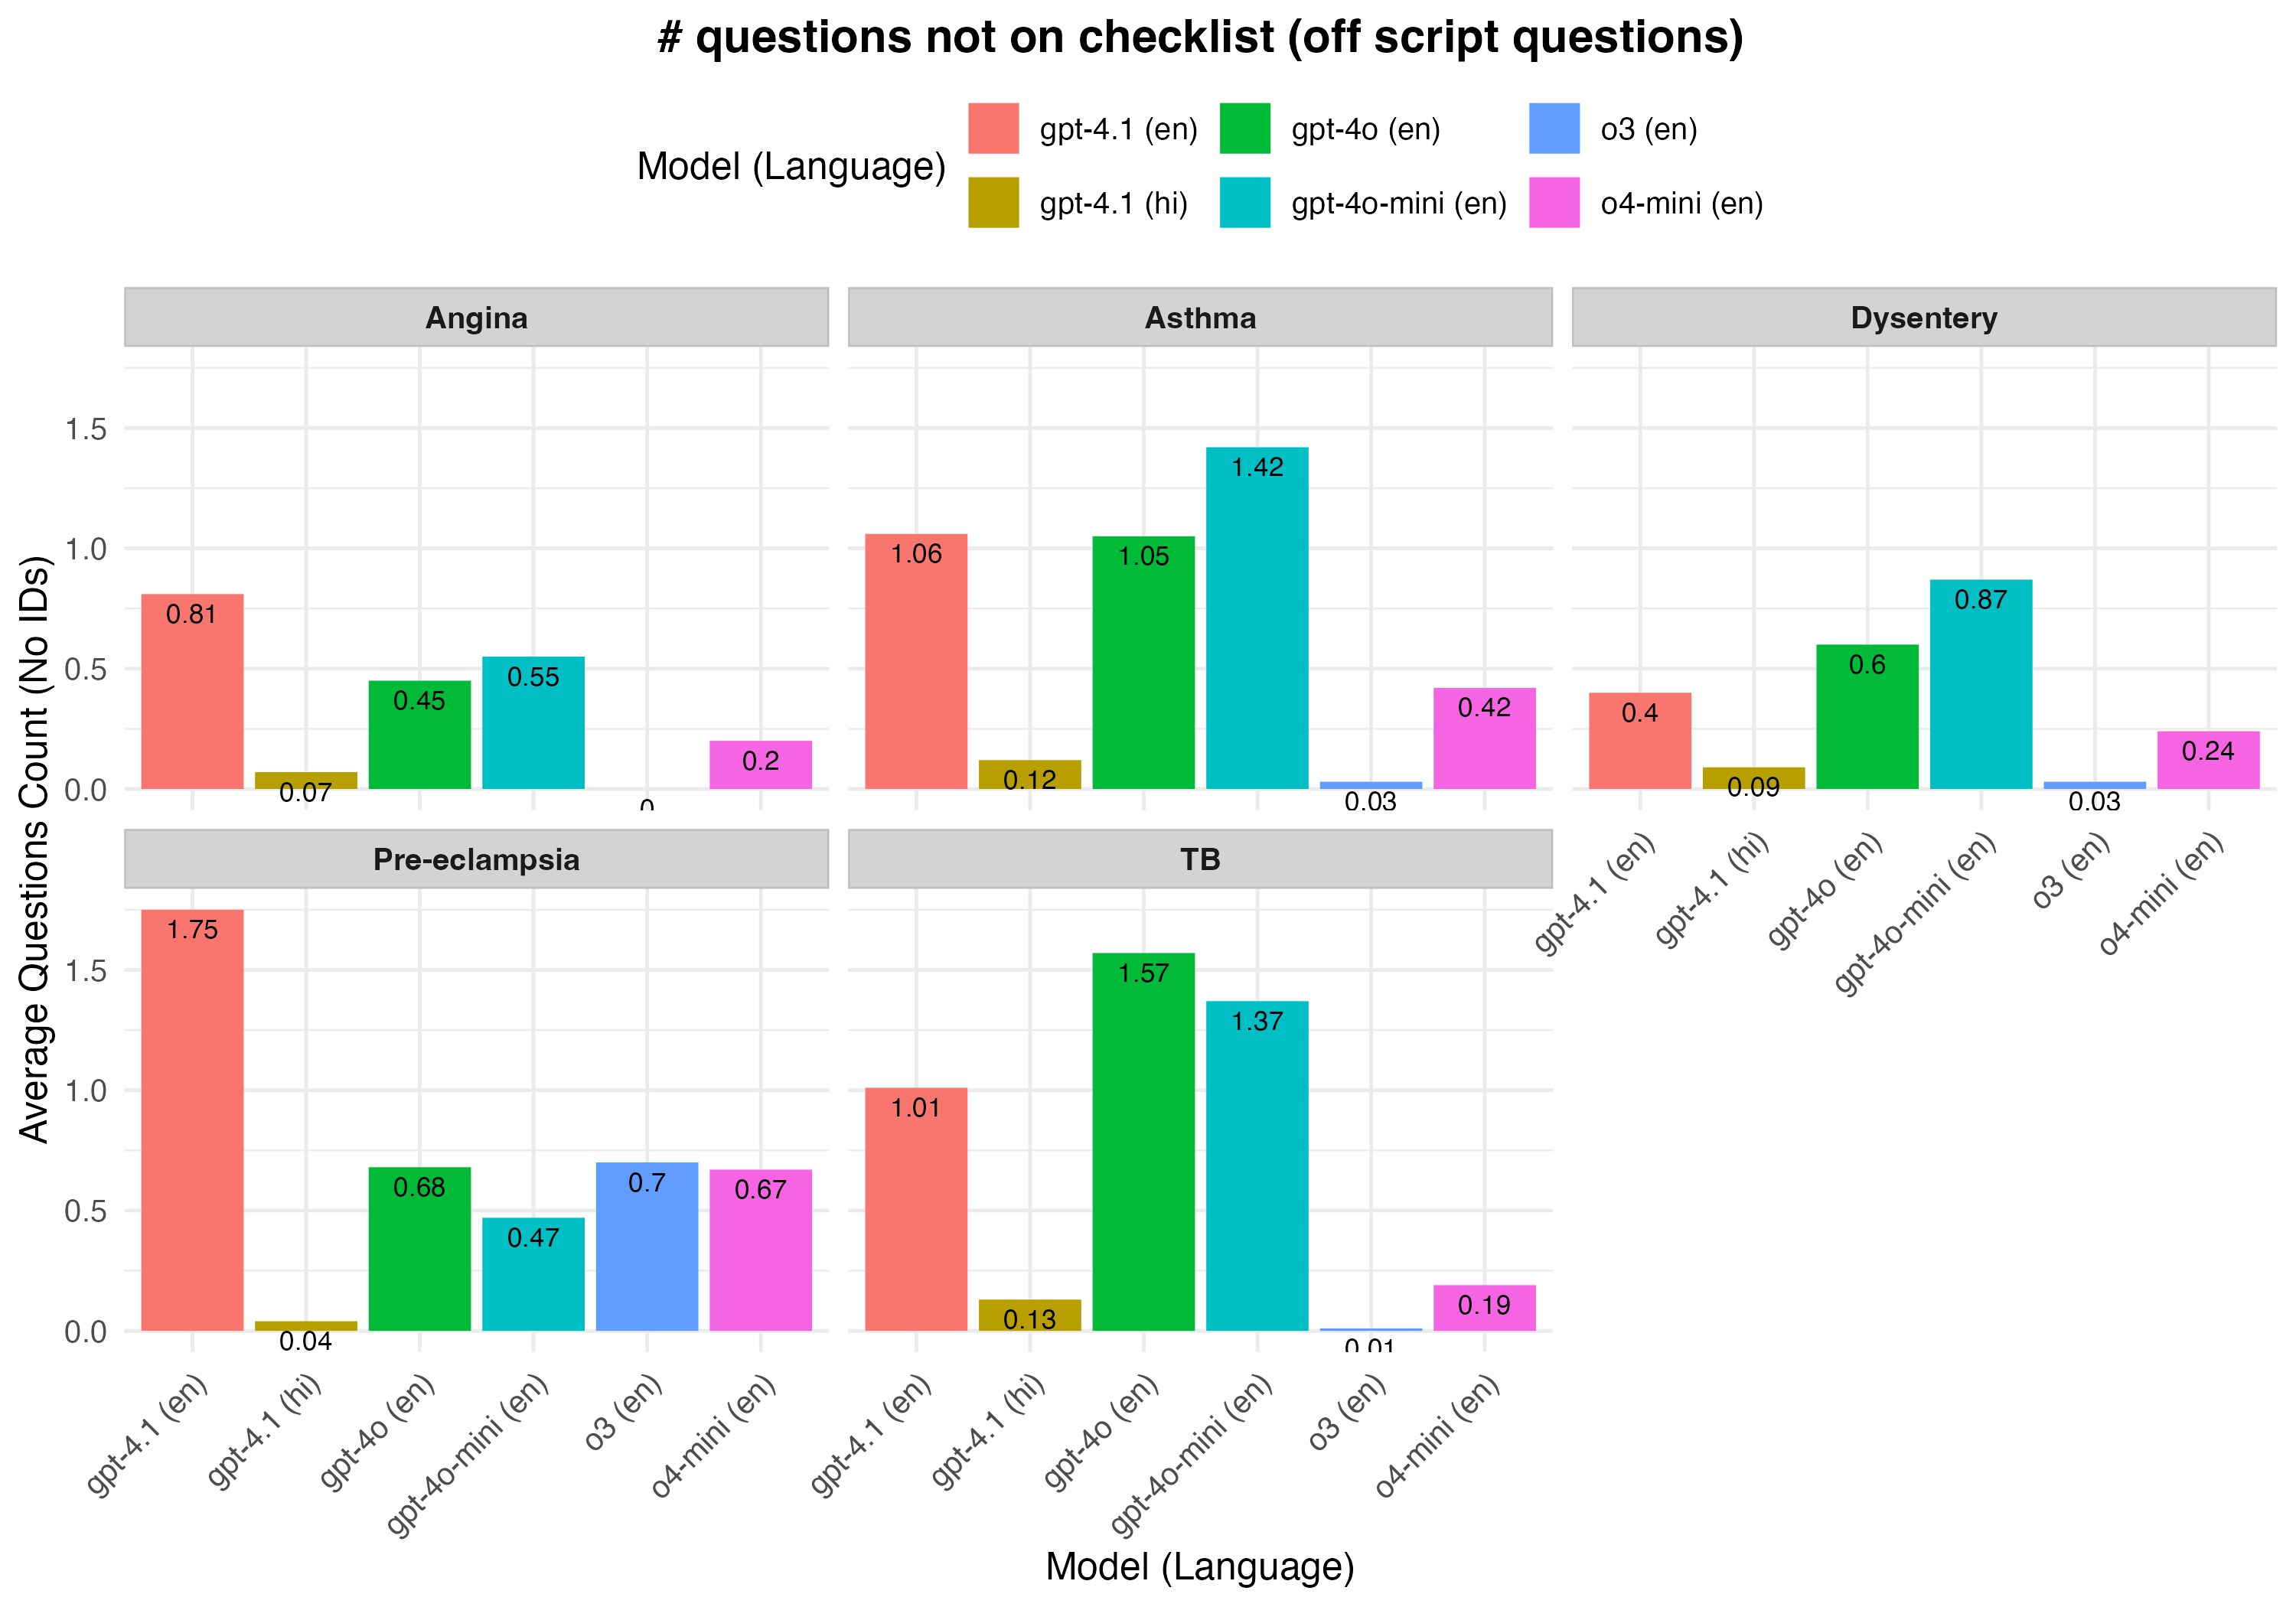
\includegraphics[width=0.9\textwidth]{figs/doctor_questions_without_ids_plot.png}
    \caption{Bar plot of the number of questions not on the checklist (off-script questions), faceted by case.}
    \label{fig:doc_questions_no_ids}
\end{figure}
\newpage

\section{Diagnosis Classification Proportions}
\begin{figure}[h!]
    \centering
    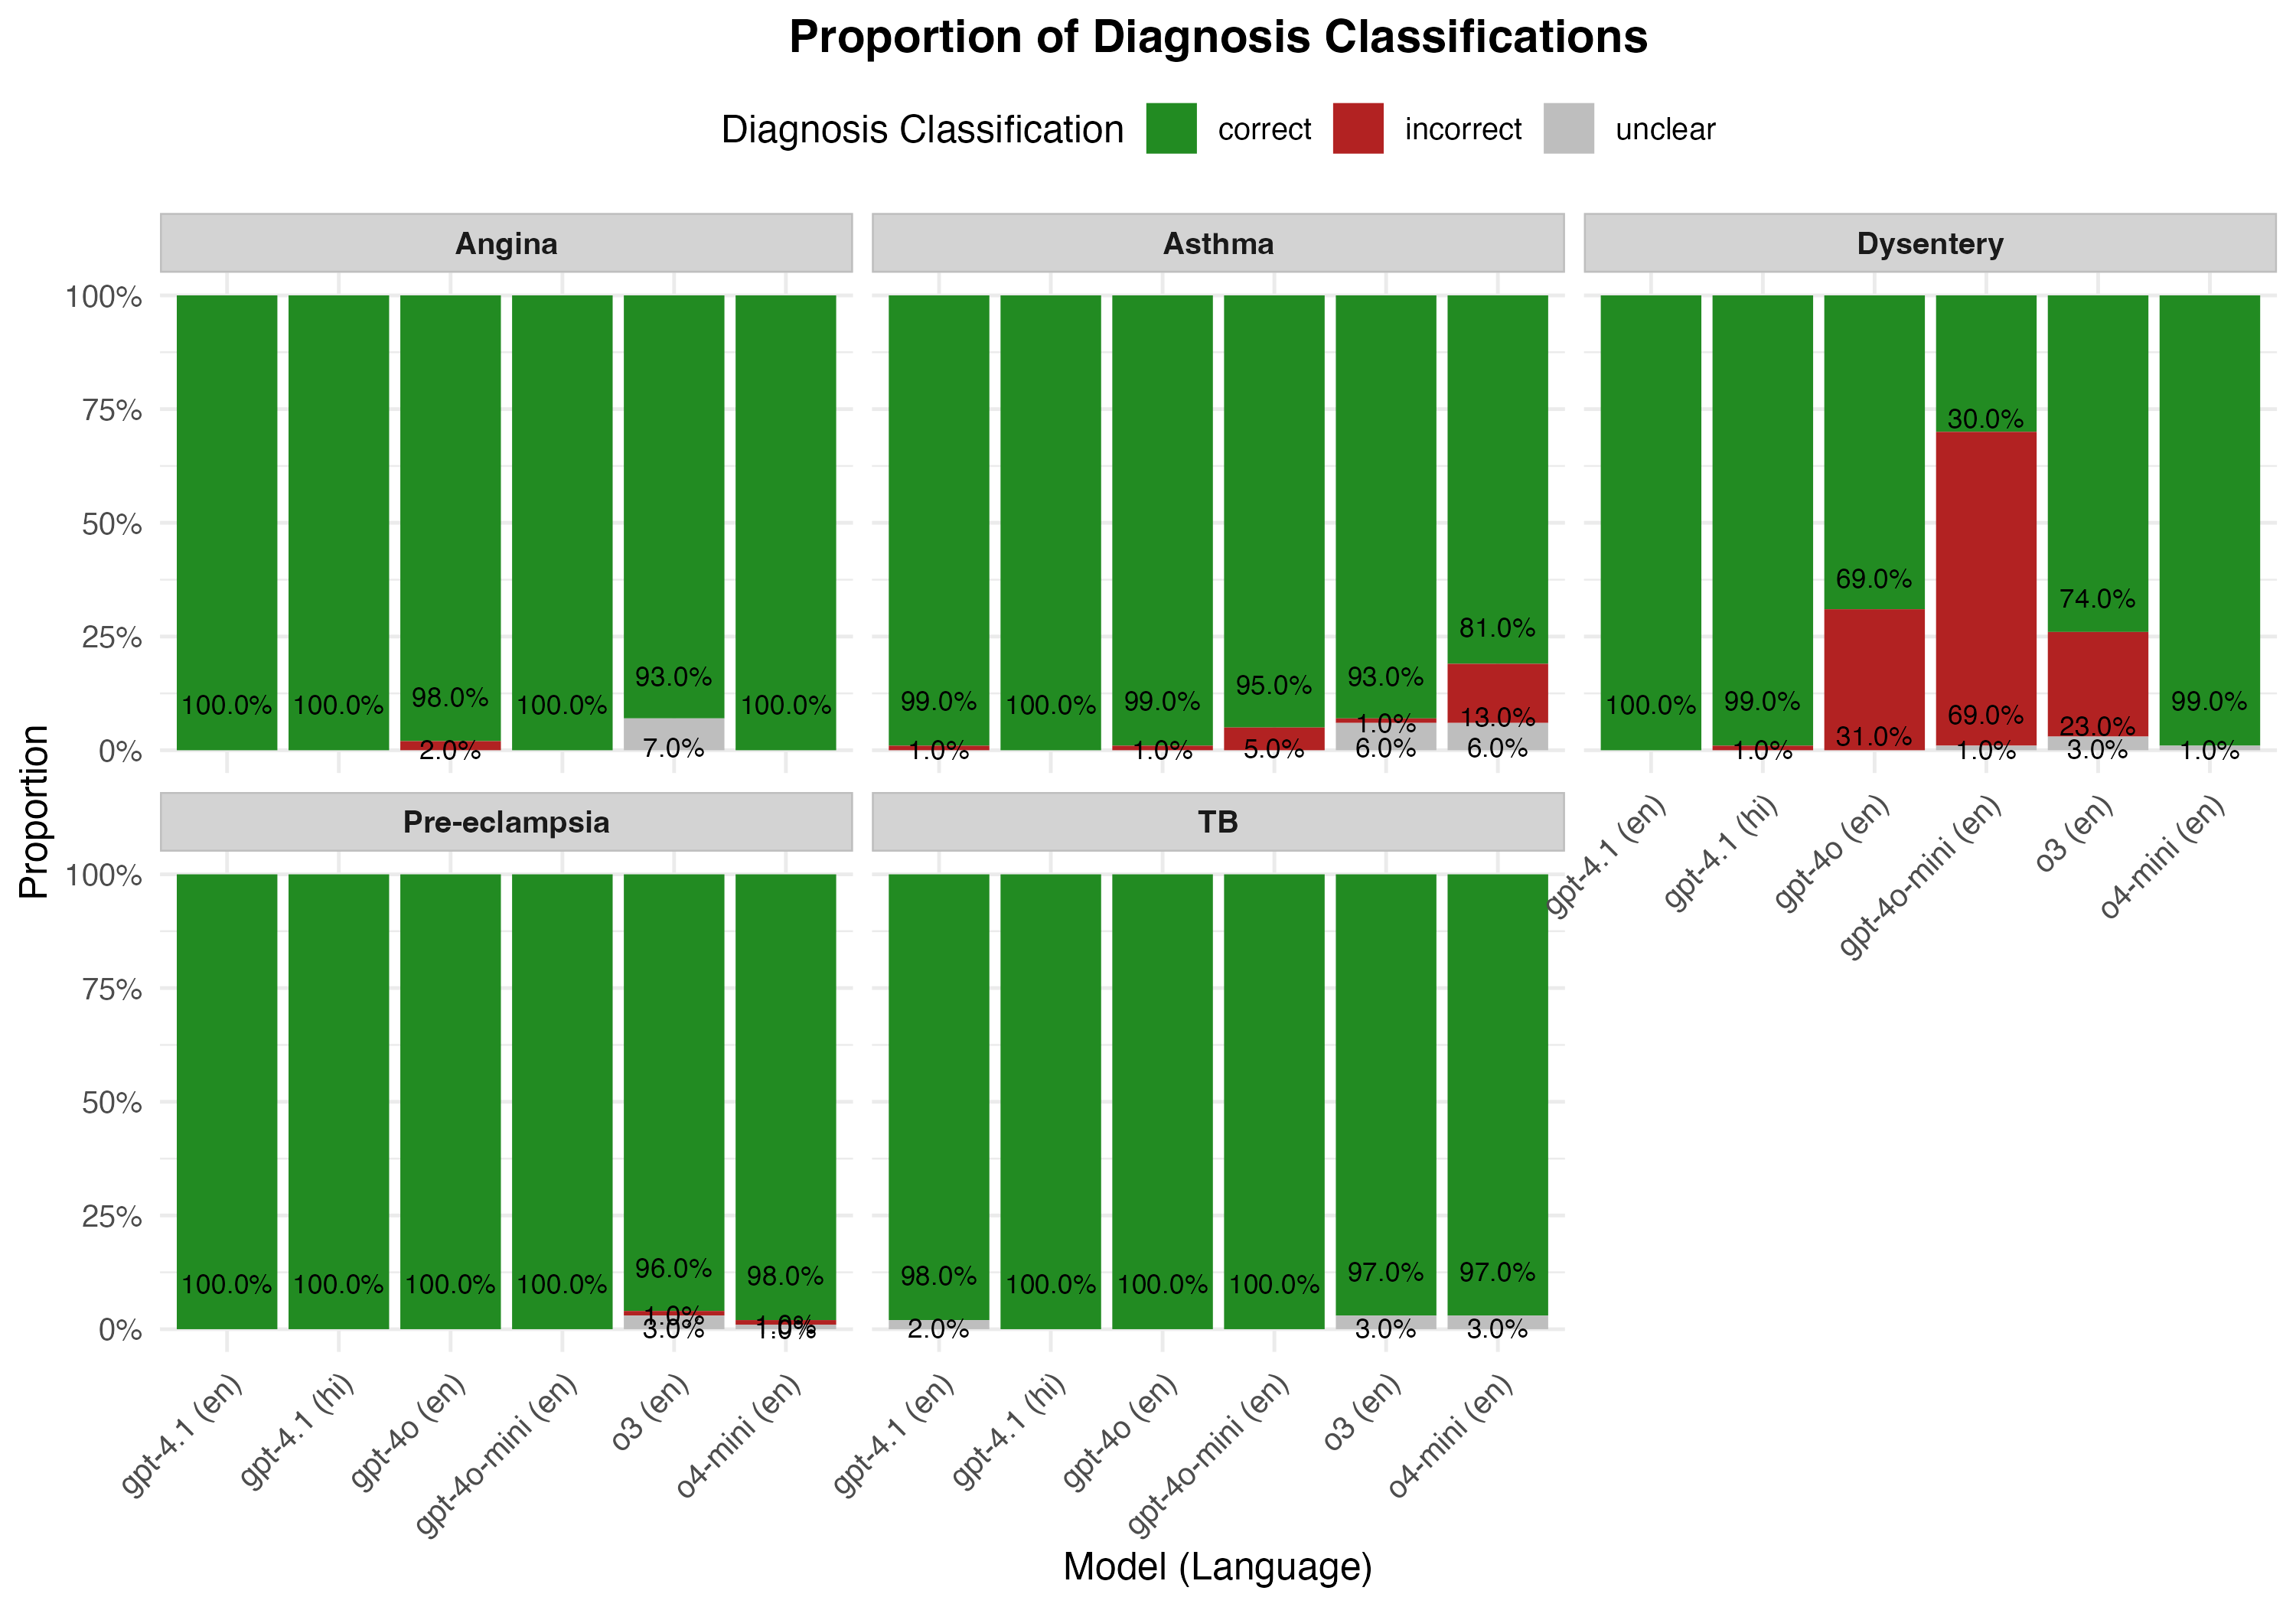
\includegraphics[width=0.9\textwidth]{figs/diag_classification_proportions_plot.png}
    \caption{Proportion of diagnosis classifications (correct, incorrect, unclear), faceted by case.}
    \label{fig:diag_classification}
\end{figure}
\newpage

\section{Treatment Proportions}
\begin{figure}[h!]
    \centering
    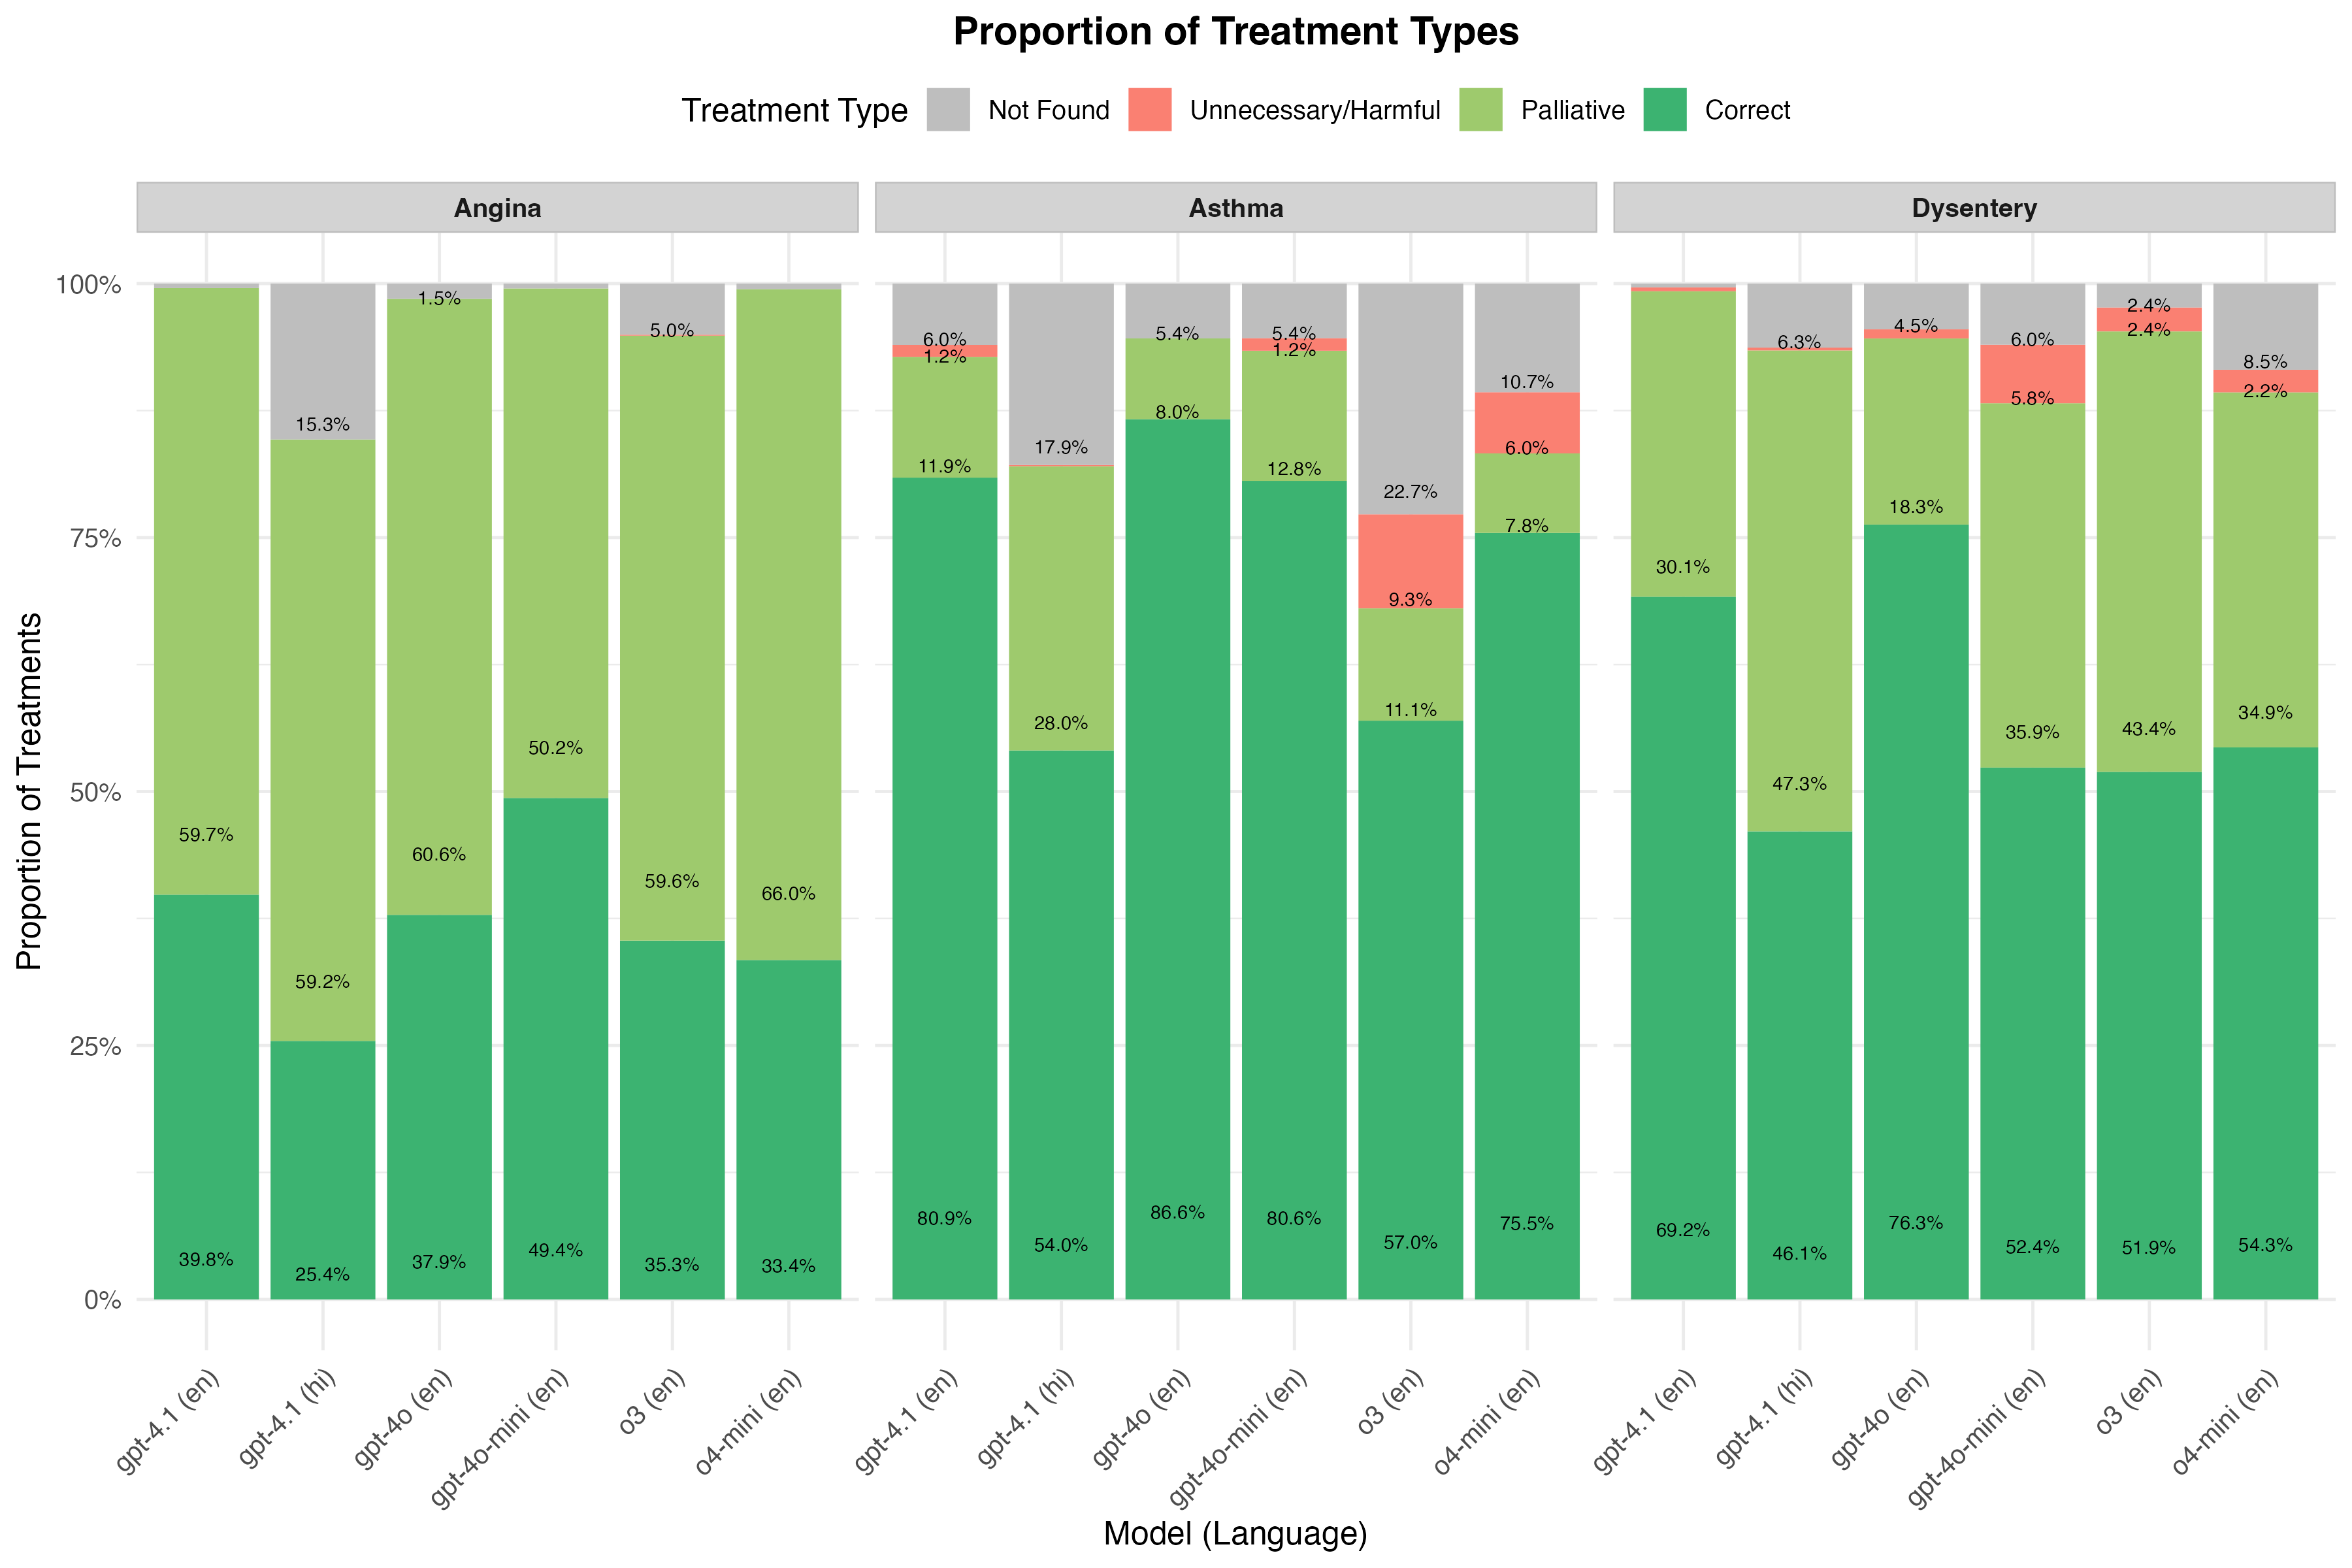
\includegraphics[width=0.9\textwidth]{figs/treatment_proportions_plot.png}
    \caption{Proportion of treatment types (Correct, Palliative, Unnecessary/Harmful, Not Found), faceted by case.}
    \label{fig:treatment_proportions}
\end{figure}

\end{document} 